\documentclass[t,aspectratio=169]{beamer}

\usepackage{soul}
\usepackage{multicol}
\usepackage[utf8]{inputenc}

\usepackage{amsmath}
\usepackage{physics}
\usepackage{siunitx}
\usepackage{graphicx}


% ----------------------------------------------------------------------------------------------------------------------------------------

\title{
\includegraphics[width=45pt]{oepecsetlogo.png}\\(KTXFI2EBNF) Physics II. Lecture}

% \subtitle{1-4. lecture}

\author{Dr.~Gábor FACSKÓ, PhD\\\tiny Assistant Professor / Senior Research Fellow\\\textit{facsko.gabor@uni-obuda.hu}}

\institute{\Tiny Óbuda University, Faculty of Electrical Engineering, 1084 Budapest, Tavaszmező u. 17.\\Wigner Research Centre for Physics, Department of Space Physics and Space Technology, 1121 Budapest, Konkoly-Thege Miklós út 29–33.\\ \url{https://wigner.hu/~facsko.gabor}}

\date{October 20,~2025}

\logo{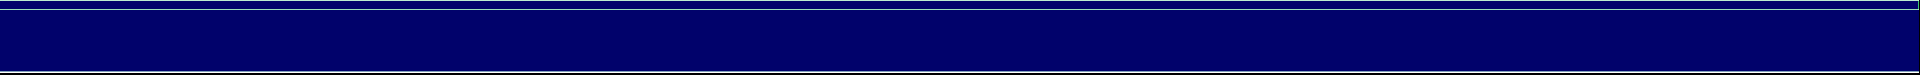
\includegraphics[height=0.9 true cm]{kekcsik.png}}

% ----------------------------------------------------------------------------------------------------------------------------------------

\begin{document}

\frame{\titlepage}

% ----------------------------------------------------------------------------------------------------------------------------------------

\begin{frame}[fragile,squeeze,allowframebreaks]
\frametitle{Where are we?}
\begin{itemize}
\setlength{\parskip}{0pt}
\setlength{\itemsep}{0pt}
\item \st{Motion of charged particles in electromagnetic fields.}
\item \st{Elements of quantum mechanics. Heisenberg's uncertainty principle. The stationary Schrödinger equation and its applications.}
\item \st{Limits of the classical conceptual framework. Thermal radiation. Photoelectric effect. Compton effect. The dual nature of electromagnetic radiation. The dual nature of particles.}
\item \st{Moving reference frames. Inertial forces in accelerating reference frames. Elements of special relativity. Dirac-equation, antimatter.}
\item \textbf{The classical theory of atomic structure (Rutherford, Franck-Hertz experiment, Bohr model, quantum numbers, Pauli exclusion principle).}
\item Physics of condensed matter. Metallic bonding. Electrical conduction in metals based on the free electron model and the wave model. Hall effect. Band theory of solids.
\pagebreak
\item Semiconductors. Elements of Fermi-Dirac statistics. Thermoelectric phenomena. Magnetic properties.  
\item Ferroelectricity. Piezoelectricity and electrostriction. Liquid crystals. Superconductivity.
\item Luminescence. Lasers. Basic knowledge of nuclear physics. Basic knowledge of particle physics.
\end{itemize}
\end{frame}

% ----------------------------------------------------------------------------------------------------------------------------------------

\begin{frame}[fragile,squeeze,allowframebreaks]
\frametitle{Atomic Models, Quantum Numbers, and Pauli Exclusion Principle}
\begin{columns}
  \begin{column}{0.3\textwidth} 
\begin{center}
\includegraphics[width=0.95\textwidth]{images-20251020/plumpudding.jpg}
\end{center}
\end{column}
\begin{column}{0.45\textwidth}
 \begin{itemize}
\setlength{\parskip}{0pt}
\setlength{\itemsep}{0pt}
\item Plum Pudding Model
  \begin{itemize}
    \item \textbf{J.J. Thomson (1897):} The atom’s “plum pudding” model.
    \item The atom is overall neutral: positive charge distributed uniformly in a sphere.
    \item Analogy:
    \begin{itemize}
        \item Dough $\rightarrow$ positive charge
        \item Raisins $\rightarrow$ negative electrons
    \end{itemize}
  \end{itemize}
\end{itemize}
\end{column}
\end{columns}
\pagebreak
\begin{columns}
  \begin{column}{0.55\textwidth} 
\begin{center}
\includegraphics[width=0.95\textwidth]{images-20251020/Rutherfords-Experiment-Size-of-the-Nucleus-3.png}
\end{center}
\end{column}
\begin{column}{0.45\textwidth}
\begin{itemize}
\setlength{\parskip}{0pt}
\setlength{\itemsep}{0pt}
\item Rutherford Atomic Model (1909–1911)
\begin{itemize}
    \item University of Manchester: Hans Geiger, Ernest Marsden under the direction of Ernest Rutherford.
   \item Gold foil scattering experiment using alpha particles.
   \item \textbf{Expected:} Alpha particles pass through with small deflections.
\item \textbf{Observed:} Some alpha particles scattered at large angles.
   \end{itemize}
 \end{itemize}
\end{column}
\end{columns}
\pagebreak
\begin{columns}
  \begin{column}{0.6\textwidth} 
\begin{center}
\includegraphics[width=0.95\textwidth]{images-20251020/rutherford.png}
\end{center}
\end{column}
\begin{column}{0.4\textwidth}
\begin{itemize}
\setlength{\parskip}{0pt}
\setlength{\itemsep}{0pt}
\item Explanation of the experiment
\begin{itemize}
\item If the atom followed the Plum Pudding Model, alpha particles would not scatter strongly.
\item Observation implies the existence of a massive, positively charged, localized scattering center -  the nucleus.
  \end{itemize}
\end{itemize}
\end{column}
\end{columns}
\pagebreak
\begin{itemize}
\setlength{\parskip}{0pt}
\setlength{\itemsep}{0pt}
\item Rutherford Model Characteristics
\begin{itemize}
    \item The atom’s mass is concentrated in the nucleus.
    \item Electrons revolve in circular orbits held by electrostatic (Coulomb) attraction.
    \item \textbf{Flaw:} Accelerating charges radiate energy $\rightarrow$ the electron would spiral into the nucleus.
    \item Since this does not occur, the model is incomplete.
    \end{itemize}
\end{itemize}
\pagebreak
\begin{itemize}
\setlength{\parskip}{0pt}
\setlength{\itemsep}{0pt}
\item Spectral Analysis
\begin{center}
%ource $\rightarrow$ Optical grating $\rightarrow$ Mirrors $\rightarrow$ Detector
  \includegraphics[width=0.9\textwidth]{images-20251020/spectral.png}
\end{center}
\pagebreak
\item Precursors to the Bohr Model
\begin{itemize}
    \item \textbf{Johann Balmer (1825–1898):} Hydrogen shows a line spectrum.
    $$     \frac{1}{\lambda} = R_H \left( \frac{1}{2^2} - \frac{1}{n^2} \right), \quad n = 3, 4, 5, \dots $$
    \item \textbf{Johannes Rydberg (1854–1919):} Extended formula to other atoms.
      $$     \frac{1}{\lambda} = R_H \left( \frac{1}{n_1^2} - \frac{1}{n_2^2} \right) $$
 \end{itemize}
\pagebreak
  \item \textbf{Franck–Hertz Experiment:} Mercury atoms absorb discrete energies, e.g. $h f = 4.9\,\text{eV}$.
     \begin{center}
    \includegraphics[width=0.4\textwidth]{images-20251020/franckhertz-a.png}
    \includegraphics[width=0.4\textwidth]{images-20251020/franckhertz-b.png}
  \end{center}
\pagebreak
  \item Spectra: H, He, and Ne atoms, respectively \medskip
     \begin{center}
   \includegraphics[width=0.35\textwidth]{images-20251020/spectra.png}
  \end{center}
\pagebreak
\item Bohr Atomic Model
\begin{itemize}
    \item Atoms exist in stationary states with definite energies $E_1, E_2, \dots$ — no radiation occurs.
    \item Electrons orbit the nucleus only on specific paths with discrete energies.
    \end{itemize}
    \medskip
  \begin{center}
   \includegraphics[width=0.6\textwidth]{images-20251020/bohr.jpg}
  \end{center}
\pagebreak
\item Bohr Model: Energy Transitions
\begin{itemize}
    \item Transition between levels involves photon emission or absorption:
    $$     W_n - W_k = h f $$
    \item The photon energy equals the energy difference between levels.
    \end{itemize}
 \medskip
  \begin{center}
    \includegraphics[width=0.4\textwidth]{images-20251020/excitement.jpg}
 \end{center}
\pagebreak
\item Bohr Model: Quantization of Angular Momentum
\begin{align*}
    m r v &= n \frac{h}{2\pi} = n \hbar
\end{align*}
\begin{itemize}
    \item Only orbits where the electron’s angular momentum is an integer multiple of $\hbar$ are allowed.
    \item \textbf{Principal quantum number:} $n$
    \end{itemize}
\pagebreak
\item Bohr–Sommerfeld Model
\begin{itemize}
    \item Fine structure of spectral lines observed.
    \item Sommerfeld introduced elliptical orbits: $$ L = l \frac{h}{2\pi} $$
    \item \textbf{Azimuthal (orbital) quantum number:} $l = 0, 1, 2, \dots, n-1$
    \end{itemize}
    \pagebreak
\item Zeeman Effect
\begin{itemize}
    \item \textbf{Pieter Zeeman (1865–1943):}
    \item In a strong magnetic field, spectral lines split into components — the normal Zeeman effect.
    \end{itemize}
\medskip
  \begin{center}
    \includegraphics[width=0.35\textwidth]{images-20251020/zeeman-a.png}
    \includegraphics[width=0.2\textwidth]{images-20251020/zeeman-b.jpg}
     \includegraphics[width=0.35\textwidth]{images-20251020/zeeman-c.jpg}
 \end{center}
\pagebreak
\begin{columns}
  \begin{column}{0.35\textwidth} 
\begin{center}
\includegraphics[width=0.95\textwidth]{images-20251020/bohrmagneton.png}
\end{center}
\end{column}
\begin{column}{0.6\textwidth}
\item Magnetic Quantum Number
\begin{itemize}
    \item Bohr magneton: $M_B = \dfrac{e h}{4 \pi m_e}$
    \item Magnetic dipole moment: $M = M_B l$
    \item z-component: $M_z = M_B l \cos \alpha$
    \item \textbf{Magnetic quantum number:} $m = -l, \dots, 0, \dots, +l$
    \end{itemize}
\item Spin 
\begin{itemize}
    \item Spin angular momentum: $L_S = \pm \dfrac{1}{2} \dfrac{h}{2\pi}$
    \item \textbf{Spin quantum number:} $s = \pm \dfrac{1}{2}$
    \end{itemize}
\end{column}
\end{columns}

\pagebreak
\item Pauli Exclusion Principle
\begin{itemize}
    \item No two electrons in an atom can share the same set of four quantum numbers.
    \item Only one electron can occupy a given quantum state.
    \end{itemize}
    \pagebreak
  \item Electron structure
    \smallskip
    \begin{center}
\includegraphics[width=0.7\textwidth]{images-20251020/spdf.jpg}
\end{center}
\pagebreak
\smallskip
\begin{center}
\includegraphics[width=0.75\textwidth]{images-20251020/quantumnumbers.png}
\end{center}
\pagebreak
\begin{center}
  \includegraphics[width=0.85\textwidth]{images-20251020/PeriodicTableECBlocks.png}
  \end{center}
  \pagebreak
  \begin{center}
    \begin{tabular*}{1.0\linewidth}{rl}
        \includegraphics[width=0.3\textwidth]{images-20251020/atomicorbits.png}
      &
        \includegraphics[width=0.23\textwidth]{images-20251020/atomicorbits2.jpg} \\
       \includegraphics[width=0.6\textwidth]{images-20251020/atomicorbits4.png}
  &
  \includegraphics[width=0.23\textwidth]{images-20251020/atomicorbits3.png}
    \end{tabular*} 
\end{center}
\end{itemize}
\end{frame}

%------------------------------------------------

\begin{frame}[fragile,squeeze,allowframebreaks]
 \frametitle{Wave–Particle Duality}
 \begin{itemize}
   \setlength{\parskip}{0pt}
\setlength{\itemsep}{0pt}
 \item Light and matter exhibit both particle and wave properties.
 \item De Broglie Matter-Wave Theory
\begin{itemize}
    \item \textbf{Louis de Broglie (1892–1987):}
    \item Based on light’s dual nature, proposed that particles have wavelength: $$ \lambda = \frac{h}{p} = \frac{h}{m v} $$
    \item \textbf{De Broglie wavelength:} $\lambda = h / p$
    \item Verified by the Davisson–Germer experiment (electron diffraction).
    \end{itemize}
 \pagebreak
\item Wave–Particle Demonstrations
 \smallskip
\begin{center}
  \includegraphics[width=0.6\textwidth]{images-20251020/pwave-a.jpg}\\
  1 slit + light $\rightarrow$ particle pattern
\end{center}
\pagebreak
\begin{center}
  \includegraphics[width=0.65\textwidth]{images-20251020/pwave-b.jpg} \\
  1 slit + light $\rightarrow$ waves
\end{center}
\pagebreak
\begin{center}
  \includegraphics[width=0.65\textwidth]{images-20251020/pwave-c.jpg}\\
  2 slits + light $\rightarrow$ interference fringes
\end{center}
\pagebreak
\begin{center}
  \includegraphics[width=0.65\textwidth]{images-20251020/pwave-d.jpg}\\
  2 slits + light $\rightarrow$ interference fringes
\end{center}
\pagebreak
\begin{center}
  \includegraphics[width=0.65\textwidth]{images-20251020/pwave-e.jpg}\\
  1 slit + electron $\rightarrow$ particle pattern
\end{center}
\pagebreak
\begin{center}
  \includegraphics[width=0.75\textwidth]{images-20251020/pwave-f.jpg}\\
  2 slits + electrons $\rightarrow$ interference pattern\\
  \end{center}
\pagebreak
\begin{center}
  \includegraphics[width=0.65\textwidth]{images-20251020/pwave-g.jpg}\\
2 slits + electrons $\rightarrow$ interference pattern\\
 \textbf{Conclusion:} Electrons have wave properties!
\end{center}
\end{itemize}
\end{frame}

% ----------------------------------------------------------------------------------------------------------------------------------------
\begin{frame}[fragile,squeeze,allowframebreaks]
\frametitle{Elements of Quantum Mechanics}
\begin{itemize}
   \setlength{\parskip}{0pt}
\setlength{\itemsep}{0pt}
 \item Fundamental principles governing atomic and subatomic systems.
\item Heisenberg Uncertainty Principle
  \begin{itemize}
    \item Certain pairs of quantities (e.g. position and momentum) cannot be measured simultaneously with arbitrary precision.
    \item \textbf{Relations:} $$  \Delta t \, \Delta E \geq h, \qquad \Delta x \, \Delta p \geq h $$
   \end{itemize}
\pagebreak
\item Heisenberg’s first uncertainty principle: $$t=\frac{1}{f}\Rightarrow \Delta t \ge \frac{1}{f}$$ $$W=h\cdot f \Rightarrow \Delta W=h\cdot \Delta f \Rightarrow \frac{1}{\Delta f}=\frac{h}{\Delta W},$$ therefore, $\Delta t\le\frac{h}{\Delta W}$. So, $$\Delta t\cdot\Delta W \le h.$$
In the physical description of micro-objects, the product of the uncertainties in energy and time cannot be smaller than Planck’s constant.  
Example: The exact energy of a photon could only be determined from measurements carried out over an infinitely long period.
  \pagebreak
\item Heisenberg’s second uncertainty principle: $f=\frac{\nu}{\lambda}\Rightarrow$ the finite difference with respect to $\lambda$: $\frac{\Delta f}{\Delta \lambda}=-\frac{\nu}{\lambda^{2}}.$\\
Rearranging: $$-\frac{\Delta f\cdot\lambda^{2}}{\Delta\lambda}=\nu$$ $$-\frac{\lambda^{2}}{\Delta\lambda}=\frac{\nu}{\Delta f}.$$
The de Broglie equation: $p = \frac{h}{\lambda}$.
Take the finite difference with respect to $\lambda$: $\frac{\Delta p}{\Delta\lambda}=-\frac{h}{\lambda^{2}}$.\\
Rearranging:
$$-\frac{\Delta p\cdot\lambda^{2}}{\Delta\lambda}=h$$
\pagebreak
$$-\frac{\lambda^{2}}{\Delta\lambda}=\frac{h}{\Delta p}.$$
\item Heisenberg’s second uncertainty principle: $$-\frac{\lambda^{2}}{\Delta\lambda}=\frac{\nu}{\Delta f}$$ and $$-\frac{\lambda^{2}}{\Delta\lambda}=\frac{h}{\Delta p}.$$
  Therefore $$\frac{\nu}{\Delta f}=\frac{h}{\Delta p}.$$
  \pagebreak
  So, $$v\cdot\Delta t\ge\frac{h}{\Delta p}.$$
  However, $$v\cdot\Delta t=\Delta x,$$ hence: $$\Delta x\ge\frac{h}{\Delta p'},$$ or $$\Delta x\cdot\Delta p \ge h.$$
  In the physical description of micro-objects, the product of the uncertainties of momentum and position cannot be smaller than Planck’s constant.\\

  Example: the orbit of an electron cannot be precisely described. We cannot, for instance, determine its exact velocity at a given position.
 \pagebreak
\item Bohr’s Complementarity Principle
\begin{itemize}
    \item Wave and particle properties are complementary aspects of microscopic objects.
    \item Both are needed for a complete description.
    \end{itemize}
    \begin{center}
      \includegraphics[width=0.9\textwidth]{images-20251020/waveparticle.png}
    \end{center}
\end{itemize}
\end{frame}


% ----------------------------------------------------------------------------------------------------------------------------------------

\begin{frame}[fragile,squeeze,allowframebreaks]
\frametitle{The Dirac Equation and Its Physical Meaning}
\begin{itemize}
\setlength{\parskip}{3pt}
\setlength{\itemsep}{3pt}

\item \underline{Dirac equation (in covariant form):}
$$\left( i \hbar \gamma^{\mu} \partial_{\mu} - m c \right) \psi = 0$$

\item \underline{Explanation of symbols:}
\begin{itemize}
\item $\psi$ : Dirac spinor (a four-component wave function describing spin-$\tfrac{1}{2}$ particles, e.g. electrons)
\item $m$ : rest mass of the particle
\item $c$ : speed of light in vacuum
\item $\hbar$ : reduced Planck constant ($\hbar = \frac{h}{2\pi}$)
\item $\partial_{\mu}$ : four-gradient operator  
      $$\partial_{\mu} = \left( \frac{1}{c}\frac{\partial}{\partial t}, -\nabla \right)$$
\item $\gamma^{\mu}$ : Dirac gamma matrices ($\mu = 0,1,2,3$), satisfying  
      $$  \{ \gamma^{\mu}, \gamma^{\nu} \} = 2 g^{\mu\nu} I, $$
      where $g^{\mu\nu}$ is the Minkowski metric tensor and $I$ is the identity matrix.
\end{itemize}

\item \underline{Alternative (Hamiltonian) form:}
$$ i \hbar \frac{\partial \psi}{\partial t} = \left( -i \hbar c\, \boldsymbol{\alpha} \cdot \nabla + \beta m c^{2} \right) \psi, $$
where $\boldsymbol{\alpha}$ and $\beta$ are $4\times4$ Dirac matrices defined by  
$\alpha^{i} = \gamma^{0}\gamma^{i}$ and $\beta = \gamma^{0}$.

\pagebreak

\item \underline{Physical meaning:}
\begin{itemize}
\item The Dirac equation unifies \textbf{quantum mechanics} and \textbf{special relativity}.
\item It correctly describes particles with \textbf{spin $\tfrac{1}{2}$} and predicts their intrinsic \textbf{magnetic moment}.
\item It naturally introduces the concept of \textbf{antimatter} — particles with the same mass but opposite charge (e.g. the positron).
\item The equation ensures that the probability density remains positive and conserved under Lorentz transformations.
\item At low velocities ($v \ll c$), it reduces to the Schrödinger equation, ensuring consistency with non-relativistic quantum mechanics.
\end{itemize}

\end{itemize}
\end{frame}

% ----------------------------------------------------------------------------------------------------------------------------------------

\begin{frame}[fragile,squeeze,allowframebreaks]
\frametitle{Consequences of the Dirac Equation}
\begin{itemize}
\setlength{\parskip}{4pt}
\setlength{\itemsep}{4pt}

\item \underline{Existence of spin:}
\begin{itemize}
\item The Dirac equation naturally describes particles with \textbf{intrinsic spin $\tfrac{1}{2}$}.
\item The spin is a purely quantum mechanical property with no classical analogue.
\item The spin arises from the four-component structure of the Dirac spinor.
\end{itemize}

\item \underline{Magnetic moment:}
\begin{itemize}
\item The equation predicts the correct magnetic moment of the electron:
\[
\boldsymbol{\mu} = g \frac{e \hbar}{2 m} \mathbf{S}, \quad \text{with } g = 2.
\]
\item This prediction agrees very closely with experimental data (after quantum electrodynamic corrections).
\end{itemize}
\pagebreak
\item \underline{Negative energy solutions:}
\begin{itemize}
\item The Dirac equation allows both positive and negative energy states: $$E = \pm \sqrt{p^{2} c^{2} + m^{2} c^{4}}.$$
\item Initially a theoretical puzzle, later interpreted as the existence of \textbf{antiparticles}.
\end{itemize}

\item \underline{Antimatter:}
\begin{itemize}
\item The negative-energy solutions correspond to particles with the same mass but opposite charge.
\item This led to the prediction — and later experimental discovery — of the \textbf{positron} in 1932 (by Carl~D.~Anderson).
\pagebreak
\item Annihilation
\begin{center}
\includegraphics[width=0.95\textwidth]{images-20251020/annihilation.png}
\end{center}
\end{itemize}

\pagebreak

\item \underline{Relativistic quantum field theory:}
\begin{itemize}
\item The Dirac equation laid the foundation for \textbf{Quantum Electrodynamics (QED)}.
\item It describes interactions between charged spin-$\tfrac{1}{2}$ particles and electromagnetic fields.
\item This framework explains atomic structure, scattering, and vacuum fluctuations with exceptional precision.
\end{itemize}

\item \underline{Summary:}
\begin{itemize}
\item The Dirac equation unifies:
  \begin{itemize}
    \item Quantum mechanics (wave–particle duality),
    \item Special relativity (Lorentz invariance),
    \item and Intrinsic spin (a fundamental property of matter).
  \end{itemize}
\item It remains one of the cornerstones of modern physics.
\end{itemize}

\end{itemize}
\end{frame}


% ----------------------------------------------------------------------------------------------------------------------------------------

\begin{frame}
%\frametitle{Minden jó, ha a vége jó}

\vfill
\begin{center}
\textbf{\huge The End}

\bigskip
Thank you for your attention!
\end{center}
\vfill
\end{frame}

\end{document}
